\testfile{patchplots}
\testsection{Triangle Patches}
\iftrue
{
\long\def\TESTS{%
	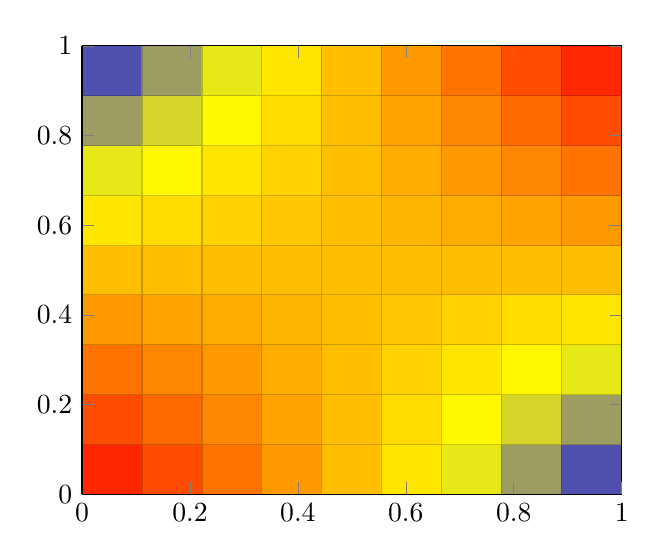
\begin{tikzpicture}
		\begin{axis}[view={0}{90}]
		\addplot3[surf,domain=0:1,samples=10] {(1-x)*(1-y) + x*y};
		\end{axis}
	\end{tikzpicture}

	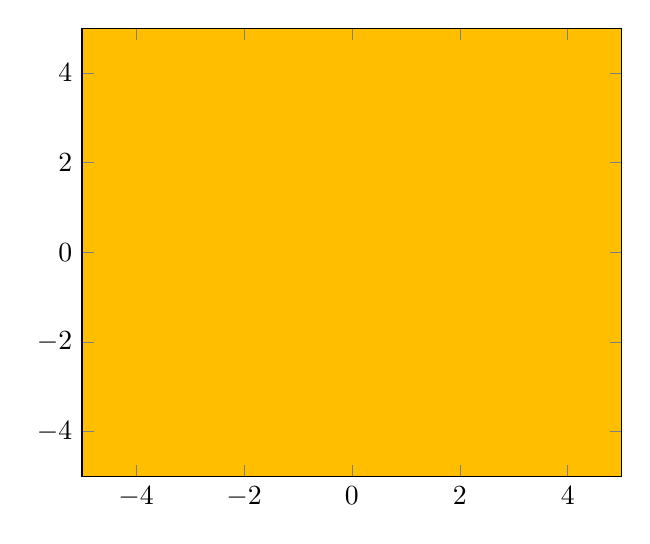
\begin{tikzpicture}
		\begin{axis}[view={0}{90}]
		\addplot3[surf,samples=2] {x*y};
		\end{axis}
	\end{tikzpicture}


	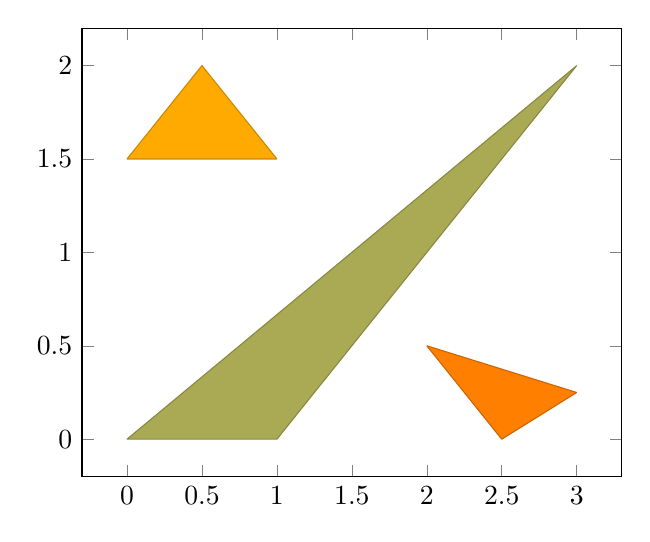
\begin{tikzpicture}
		\begin{axis}
			
		\addplot[patch,point meta=\thisrow{c}] table[row sep=\\] {
			x y c\\
			0 0 0\\
			1 0 0 \\
			3 2 2\\
			%\\
			0 1.5  1.5\\
			1 1.5  1.5\\
			0.5 2  2\\
			%\\
			2.5 0     1\\
			3 	0.25  2\\
			2 0.5     3\\
		}; 
		\end{axis}
	\end{tikzpicture}

	\begin{tikzpicture}
		\begin{axis}
		\addplot3[patch] file {plotdata/FokkerDrI_layer_0.patches.dat};
		\end{axis}
	\end{tikzpicture}



	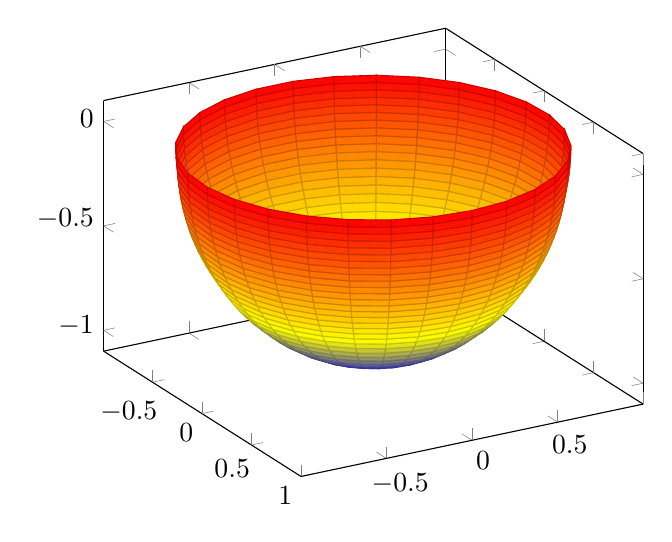
\begin{tikzpicture}
	\begin{axis}[view={60}{30}]
		\addplot3[surf,z buffer=sort,
			samples=30,domain=-1:0,y domain=0:2*pi]
			({sqrt(1-x^2) * cos(deg(y))},
			 {sqrt( 1-x^2 ) * sin(deg(y))},
			 x);
	\end{axis}
	\end{tikzpicture}

}

\testsubsection{shader=flat}
{
	\pgfplotsset{shader=flat}
	\TESTS
}

\testsubsection{shader=flat corner}
{
	\pgfplotsset{shader=flat corner}
	\TESTS
}

\testsubsection{shader=interp}
{
	\pgfplotsset{shader=interp}
	\TESTS
}

\testsubsection{shader=faceted interp}
{
	\pgfplotsset{shader=faceted interp}
	\TESTS
}
\testsubsection{Comparison with matlab (run matlab first!)}
{
	\long\def\matlabtestimg#1{%
		\IfFileExists{patchplots/#1}{%
			\includegraphics[width=10cm]{patchplots/#1}%
		}{%
			Matlab Test file `#1' does not exist, sorry. Run Matlab first.
		}%

		\nobreak
	}

	\input patchplots/patch_plot_example_section.tex
}
}
\fi

{
\pgfplotsset{show nodes/.style={nodes near coords=\coordindex,nodes near coords align={center}}}

\testsection{Linear Triangle Elements}
{
	\tikzappendtofigurename{linear}
	\begin{tikzpicture}
	\begin{axis}[enlargelimits, show nodes]
	\addplot[shader=interp,patch,point meta=explicit] coordinates {
		(0,0) [1]
		(1,0) [0]
		(1,1) [0]
	};
	\end{axis}
	\end{tikzpicture}

	\begin{tikzpicture}
	\begin{axis}[enlargelimits, show nodes]
	\addplot3[shader=interp,patch,point meta=z] coordinates {
		(0,0,1)
		(1,0,0)
		(1,1,0)
	};
	\end{axis}
	\end{tikzpicture}


	\begin{tikzpicture}
	\begin{axis}[title={Patch refines=2},enlargelimits, show nodes,patch refines=2]
	\addplot3[shader=faceted,patch,point meta=z] coordinates {
		(0,0,1)
		(1,0,0)
		(1,1,0)
	};
	\end{axis}
	\end{tikzpicture}

	\begin{tikzpicture}
	\begin{axis}[title={Patch refines=2},enlargelimits, show nodes,patch refines=2]
	\addplot3[shader=interp,patch,point meta=z] coordinates {
		(0,0,1)
		(1,0,0)
		(1,1,0)
	};
	\end{axis}
	\end{tikzpicture}

}

\testsection{Bilinear quadrilateral}
{
	\tikzappendtofigurename{bilinear}
	 \def\xA{0} \def\yA{0}
	 \def\xB{5} \def\yB{2}
	 \def\xC{5} \def\yC{4}
	 \def\xD{1} \def\yD{5}

	\begin{tikzpicture}
	\begin{axis}[title=PGFPlots bilinear (flat)]
	\addplot[patch,patch type=bilinear,point meta=explicit] coordinates {
		(\xA,\yA) [1] 
		(\xB,\yB) [0]
		(\xC,\yC) [0]
		(\xD,\yD) [0]
	};
	\pgfplotsextra{\foreach \n in {A,B,C,D} \node at (axis cs:\csname x\n\endcsname,\csname y\n\endcsname) {\n};}
	\end{axis}
	\end{tikzpicture}

	\begin{tikzpicture}
	\begin{axis}[title=PGFPlots bilinear (interp)]
	\addplot[patch,patch type=bilinear,shader=interp,point meta=explicit] coordinates {
		(\xA,\yA) [1] 
		(\xB,\yB) [0]
		(\xC,\yC) [0]
		(\xD,\yD) [0]
	};
	\pgfplotsextra{\foreach \n in {A,B,C,D} \node at (axis cs:\csname x\n\endcsname,\csname y\n\endcsname) {\n};}
	\end{axis}
	\end{tikzpicture}


	\newcommand\BILINEARSHAPE[5]{%
		\begin{tikzpicture}
			\begin{axis}[title={PGFPlots bilinear (#5)},shader=#5]
			\addplot3[patch,patch type=bilinear] coordinates {
				(0,0,#1)	
				(1,0,#2)
				(1,1,#3)
				(0,1,#4) 
			};
			\end{axis}
		\end{tikzpicture}
%
	}
	\newcommand\BILINEARSHAPES[1]{%
		\noindent
		\BILINEARSHAPE1000{#1}%
		\BILINEARSHAPE0100{#1}%

		\noindent
		\BILINEARSHAPE0010{#1}%
		\BILINEARSHAPE0001{#1}%
	}%
	\testsubsection{Shape Functions}
	{
		\testsubsubsection{interpolated}
		{
			\tikzappendtofigurename{interp}
			\BILINEARSHAPES{interp}
		}%

		\testsubsubsection{refined}
		{
			\tikzappendtofigurename{refine}
			\BILINEARSHAPES{faceted interp,patch refines=1}
		}

		\testsubsubsection{triangulated}
		{
			\tikzappendtofigurename{triang}
			\BILINEARSHAPES{faceted interp,patch to triangles}
		}
	}


	\testsubsection{Plot Expression}

	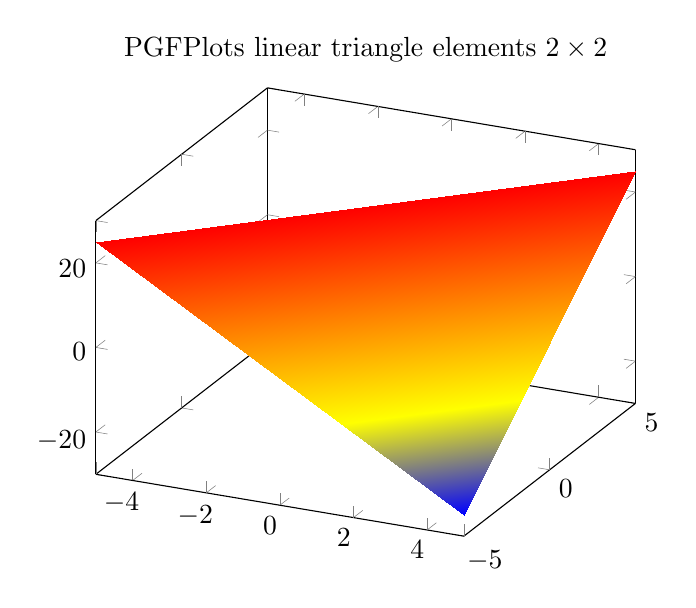
\begin{tikzpicture}
		\begin{axis}[title=rectangle,title={PGFPlots linear triangle elements $2\times 2$}]
		\addplot3[surf,shader=interp,samples=2] {x*y};
		\end{axis}
	\end{tikzpicture}

	\begin{tikzpicture}
		\begin{axis}[title=bilinear,title={PGFPlots bilinear elements $2 \times 2$}]
		\addplot3[surf,shader=interp,patch type=bilinear,samples=2] {x*y};
		\end{axis}
	\end{tikzpicture}


	{
		\pgfplotsset{patch to triangles,shader=interp,}
		\tikzappendtofigurename{triang}

		\begin{tikzpicture}
			\begin{axis}[title=bilinear,title={PGFPlots bilinear elements $2 \times 2$ triangulated}]
			\addplot3[surf,patch type=bilinear,samples=2] {x*y};
			\end{axis}
		\end{tikzpicture}

	}%
}

\testsection{Quadratic triangle}
{
	\tikzappendtofigurename{trianglequad}
	For similarly second order triangular elements beeing cut into the linear triangles (1,4,6), (4,6,5), (4,5,2) (5,6,3) as shown
	 \def\xA{0} \def\yA{0}
	 \def\xB{2} \def\yB{3}
	 \def\xC{5} \def\yC{4}
	 \def\xD{3} \def\yD{6}
	 \def\xE{0} \def\yE{7}
	 \def\xF{-1}\def\yF{4}


	\begin{tikzpicture}
	\begin{axis}[title=PGFPlots triangle quadr (flat),show nodes]
	\addplot[patch,patch type=triangle quadr,point meta=explicit] coordinates {
		(\xA,\yA) [1] 
		(\xC,\yC) [0]
		(\xE,\yE) [0]
		(\xB,\yB) [0]
		(\xD,\yD) [0]
		(\xF,\yF) [0]
	};
	\end{axis}
	\end{tikzpicture}

	\begin{tikzpicture}
	\begin{axis}[title=PGFPlots triangle quadr (interp),show nodes]
	\addplot[patch,patch type=triangle quadr,shader=interp,point meta=explicit] coordinates {
		(\xA,\yA) [1] 
		(\xC,\yC) [0]
		(\xE,\yE) [0]
		(\xB,\yB) [0]
		(\xD,\yD) [0]
		(\xF,\yF) [0]
	};
	\end{axis}
	\end{tikzpicture}


	\newcommand\QUADRATICTRI[7]{%
		\begin{tikzpicture}
		\begin{axis}[title={PGFPlots triangle quadr (#7)},
			title style={text width=8cm,align=center},
			shader=#7,show nodes]
		\addplot3[patch,patch type=triangle quadr,point meta=z] coordinates {
			(\xA,\yA,#1)
			(\xC,\yC,#2)
			(\xE,\yE,#3)
			(\xB,\yB,#4)
			(\xD,\yD,#5)
			(\xF,\yF,#6)
		};
		\end{axis}
		\end{tikzpicture}
%
		}%
	\newcommand\QUADRATICTRIANGLESHAPES[1]{%
		\noindent
		\QUADRATICTRI100000{#1}%
		\QUADRATICTRI010000{#1}%

		\noindent
		\QUADRATICTRI001000{#1}%
		\QUADRATICTRI000100{#1}%

		\noindent
		\QUADRATICTRI000010{#1}%
		\QUADRATICTRI000001{#1}%
	}

	\testsubsection{Shape Functions Interp}
	\QUADRATICTRIANGLESHAPES{interp}

	\testsubsection{Shape Functions Refined}
	{
%\tracingmacros=2 \tracingcommands=2
		\testsubsubsection{Once}
		\tikzappendtofigurename{refine}
		\QUADRATICTRIANGLESHAPES{faceted interp,mesh/refines=1}

		\testsubsubsection{twice}
		\QUADRATICTRIANGLESHAPES{faceted interp,mesh/refines=2}
	}

	\testsubsection{Shape Functions Triangulated}
	{
		\tikzappendtofigurename{triangul}
		\testsubsection{Direct: 1 Quadratic = 4 Linear}
		\QUADRATICTRIANGLESHAPES{interp,patch to triangles}

		\testsubsection{Addition Quadratic Refine: 1 Quadrate = 4 Quadratic = 16 linear}
		\QUADRATICTRIANGLESHAPES{interp,patch to triangles,mesh/refines=1}
	}

}

\testsection{Biquadratic quadrilateral}
{
	\tikzappendtofigurename{biquadratic}
	The second order quad, plotted as (1,5,8), (5,8,9), (5,9,6), (5,6,2), (3,6,7), (7,8,9), (7,9,8), (7,8,4)
	 \def\xA{0} \def\yA{0} % 1
	 \def\xB{3} \def\yB{1} % 5
	 \def\xC{6} \def\yC{1} % 2
	 \def\xD{6} \def\yD{3} % 6
	 \def\xE{5} \def\yE{5} % 3
	 \def\xF{2} \def\yF{6} % 7
	 \def\xG{-1}\def\yG{5} % 4
	 \def\xH{0} \def\yH{3} % 8

	 \def\xM{3} \def\yM{3.75} % new middle node
	 \let\xI=\xM \let\yI=\yM


	\begin{tikzpicture}
	\begin{axis}[title={PGFPlots biquadratic (flat)},show nodes]
	\addplot[patch,patch type=biquadratic,point meta=explicit] coordinates {
		(\xA,\yA) [1] 
		(\xC,\yC) [0]
		(\xE,\yE) [0]
		(\xG,\yG) [0]
		(\xB,\yB) [0]
		(\xD,\yD) [0]
		(\xF,\yF) [0]
		(\xH,\yH) [0]
		(\xI,\yI) [0]
	};
	\end{axis}
	\end{tikzpicture}

	\begin{tikzpicture}
	\begin{axis}[title=PGFPlots biquadratic (interp),show nodes]
	\addplot[patch,patch type=biquadratic,shader=interp,point meta=explicit] coordinates {
		(\xA,\yA) [1] 
		(\xC,\yC) [0]
		(\xE,\yE) [0]
		(\xG,\yG) [0]
		(\xB,\yB) [0]
		(\xD,\yD) [0]
		(\xF,\yF) [0]
		(\xH,\yH) [0]
		(\xI,\yI) [0]
	};
	\end{axis}
	\end{tikzpicture}


	\newcommand\BIQUADRATIC[9]{%
		\addplot3[] coordinates {
			(\xA,\yA,#1)  
			(\xC,\yC,#2) 
			(\xE,\yE,#3) 
			(\xG,\yG,#4) 
			(\xB,\yB,#5) 
			(\xD,\yD,#6) 
			(\xF,\yF,#7) 
			(\xH,\yH,#8) 
			(\xI,\yI,#9) 
		};
	}
	\newcommand\BIQUADRATICSHAPES[1]{{%
		\noindent
		\pgfplotsset{every axis/.style={
				patch,
				patch type=biquadratic,
				point meta=z,
				title={PGFPlots biquadratic (#1)},
				shader=#1,show nodes,
			}
		}
		\noindent
		\begin{tikzpicture}
		\begin{axis}
			\BIQUADRATIC100000000
		\end{axis}
		\end{tikzpicture}


		\noindent
		\begin{tikzpicture}
		\begin{axis}
			\BIQUADRATIC010000000
		\end{axis}
		\end{tikzpicture}

		\begin{tikzpicture}
		\begin{axis}
			\BIQUADRATIC001000000
		\end{axis}
		\end{tikzpicture}


		\noindent
		\begin{tikzpicture}
		\begin{axis}
			\BIQUADRATIC000100000
		\end{axis}
		\end{tikzpicture}

		\begin{tikzpicture}
		\begin{axis}
			\BIQUADRATIC000010000
		\end{axis}
		\end{tikzpicture}


		\noindent
		\begin{tikzpicture}
		\begin{axis}
			\BIQUADRATIC000001000
		\end{axis}
		\end{tikzpicture}

		\begin{tikzpicture}
		\begin{axis}
			\BIQUADRATIC000000100
		\end{axis}
		\end{tikzpicture}


		\noindent
		\begin{tikzpicture}
		\begin{axis}
			\BIQUADRATIC000000010
		\end{axis}
		\end{tikzpicture}

		\begin{tikzpicture}
		\begin{axis}
			\BIQUADRATIC000000001
		\end{axis}
		\end{tikzpicture}


	}}


	\BIQUADRATICSHAPES{interp}

	%\BIQUADRATICSHAPES{faceted}

	{
	\tikzappendtofigurename{triang}
	\BIQUADRATICSHAPES{interp,patch to triangles}
	}


}

}
